\documentclass[../../main.tex]{subfiles}
\begin{document}

\subsection*{7.1}
Un protone di energia cinetica $E_k = 6\ MeV$ entra in una regione di spazio in cui esiste un campo magnetico $B = 1\ T$ ortogonale al piano della traiettoria, formando con l'asse y l'angolo $\theta = 30°$.
\\Calcolare l'angolo $\theta'$ della direzione di uscita con l'asse y e la distanza lungo y tra il punto d'uscita e di ingresso.
\\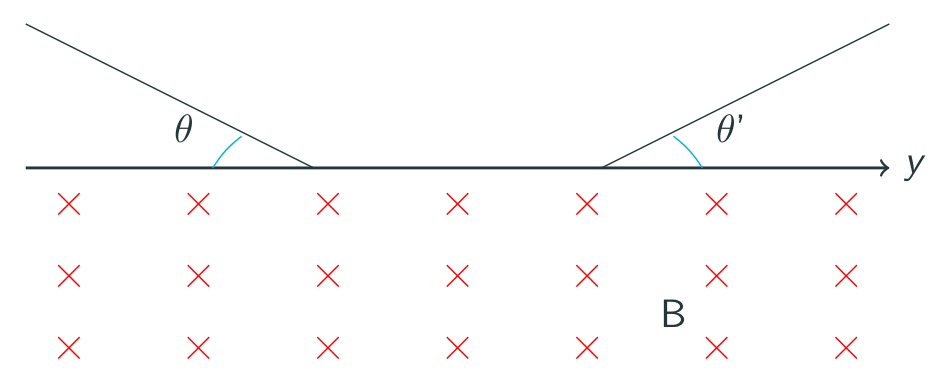
\includegraphics[scale=0.3]{e_7_1_0.png}
\\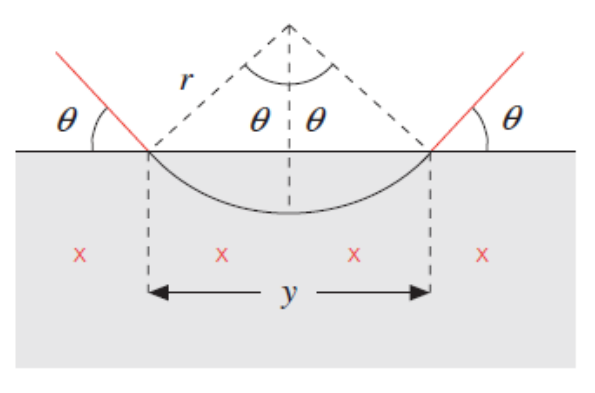
\includegraphics[scale=0.3]{e_7_1_1.png}
\subsubsection*{Formule utilizzate}
$E_K = \frac{1}{2}mv^2$
\\$|v| = \sqrt{\frac{2E_k}{m}}$
\\Forza di Lorentz sulla carica: $\vec{F}=q\vec{v}\wedge\vec{B}$
\subsubsection*{Soluzione punto a}
Dato $\vec{F}\bot \vec{s}$ 
\\$\vec{F} = m \frac{v^2}{r}\vec{u_r}$
\\$a= \frac{v^2}{r}$
\\Indico con $\alpha$ l'angolo che si forma fra il punto di entrata nel campo e il centro O.
\\$\theta + \alpha + \frac{\pi}{2} = \pi$
\\$\alpha = \pi - \frac{\pi}{2}-\theta$
\\$\beta + \alpha + \frac{\pi}{2} = \pi$
\\$\beta = \pi - \frac{\pi}{2} - \alpha = \theta$
\\$\theta' = \theta = 30°$
\\$\vec{UI} = 2\vec{IO'} = 2\vec{UO'}$
\\$\vec{IO'} = r \sin \beta = r\sin\theta$
\subsubsection*{Soluzione punto b}
$F = m\frac{v^2}{r}\vec{u_r}$   $F = q\vec{v}\wedge\vec{B}$
\\$r = \frac{mv}{qB}$ con $v=\sqrt{\frac{2E_k}{m}}$
\\$r = \frac{}{}{m}{qB}\sqrt{\frac{2E_k}{m}}=0.354\ m$
\newpage

\end{document}